% !TEX TS-program = pdflatex
% !TEX root = ../ArsClassica.tex

%************************************************
\chapter{La ricerca dei materiali (elettromeccanici)}
\label{chp:La ricerca dei materiali (elettromeccanici)}
%************************************************

\begin{tabular}{cp{1cm}p{1cm}p{1cm}} \textbf{Tipologia}&\textbf{Quantit�}&\textbf{Utilizzo}&\textbf{Risposta}\\ 
\hline \textbf{METALLI}\\
\hline Placche metallo&8&Risonatori&Ottima\\
\hline Molle a trazione Inox&2&Strumento&Sufficiente\\
\hline Molle a trazione Acciaio armonico&6&Strumento&Ottima\\
\hline Tubo Quadrato Ferro&2&Basamento&Ottima\\
\hline Viti per innesti&Varie&Bas. Attuatori&Ottima\\
\hline \textbf{VISATON - ATTUATORI}\\
\hline BSX 130 WP - 4 Ohm&4&Vibrazione Placca&Ottima\\ 
\hline ESX 45 - 8 Ohm&4&Vibrazione Placca&Sufficiente\\
\hline ESX 60 - 8 Ohm&3&Vibrazione Placca&Buona\\
\hline \textbf{MAGNETI}\\
\hline Humbucker&2&Amplificazione Molle&Buona\\
\hline Double Coil Bass&1&Amplificazione Molle&Ottima\\
\hline \textbf{PIEZOELETTRICI}\\
\hline Piezoelettrici&4&Amplificazione Molle&Buona\\
\hline 
\end{tabular}

\section{Progettazione e supporto di tiraggio}
\addcontentsline{toc}{section}{Progettazione e supporto di tiraggio}

Le molle a trazione possono arrivare ad una forza di tiraggio pari anche a 100 chili. Per questo l'utilizzo di un basamento adeguato, creato su misura da un fabbro, � la soluzione a qualunque problema relativo al paragrafo 3.3, il fissaggio di attuatori e molle.\\
Il basamento � stato creato grazie all'aiuto di un assistente del Centro di Ricerche Musicali, Leonardo Mammozzetti, che ha visionato e modificato assieme all'autore il progetto del basamento.

\begin{center}
\begin{minipage}[c]{1.\textwidth}
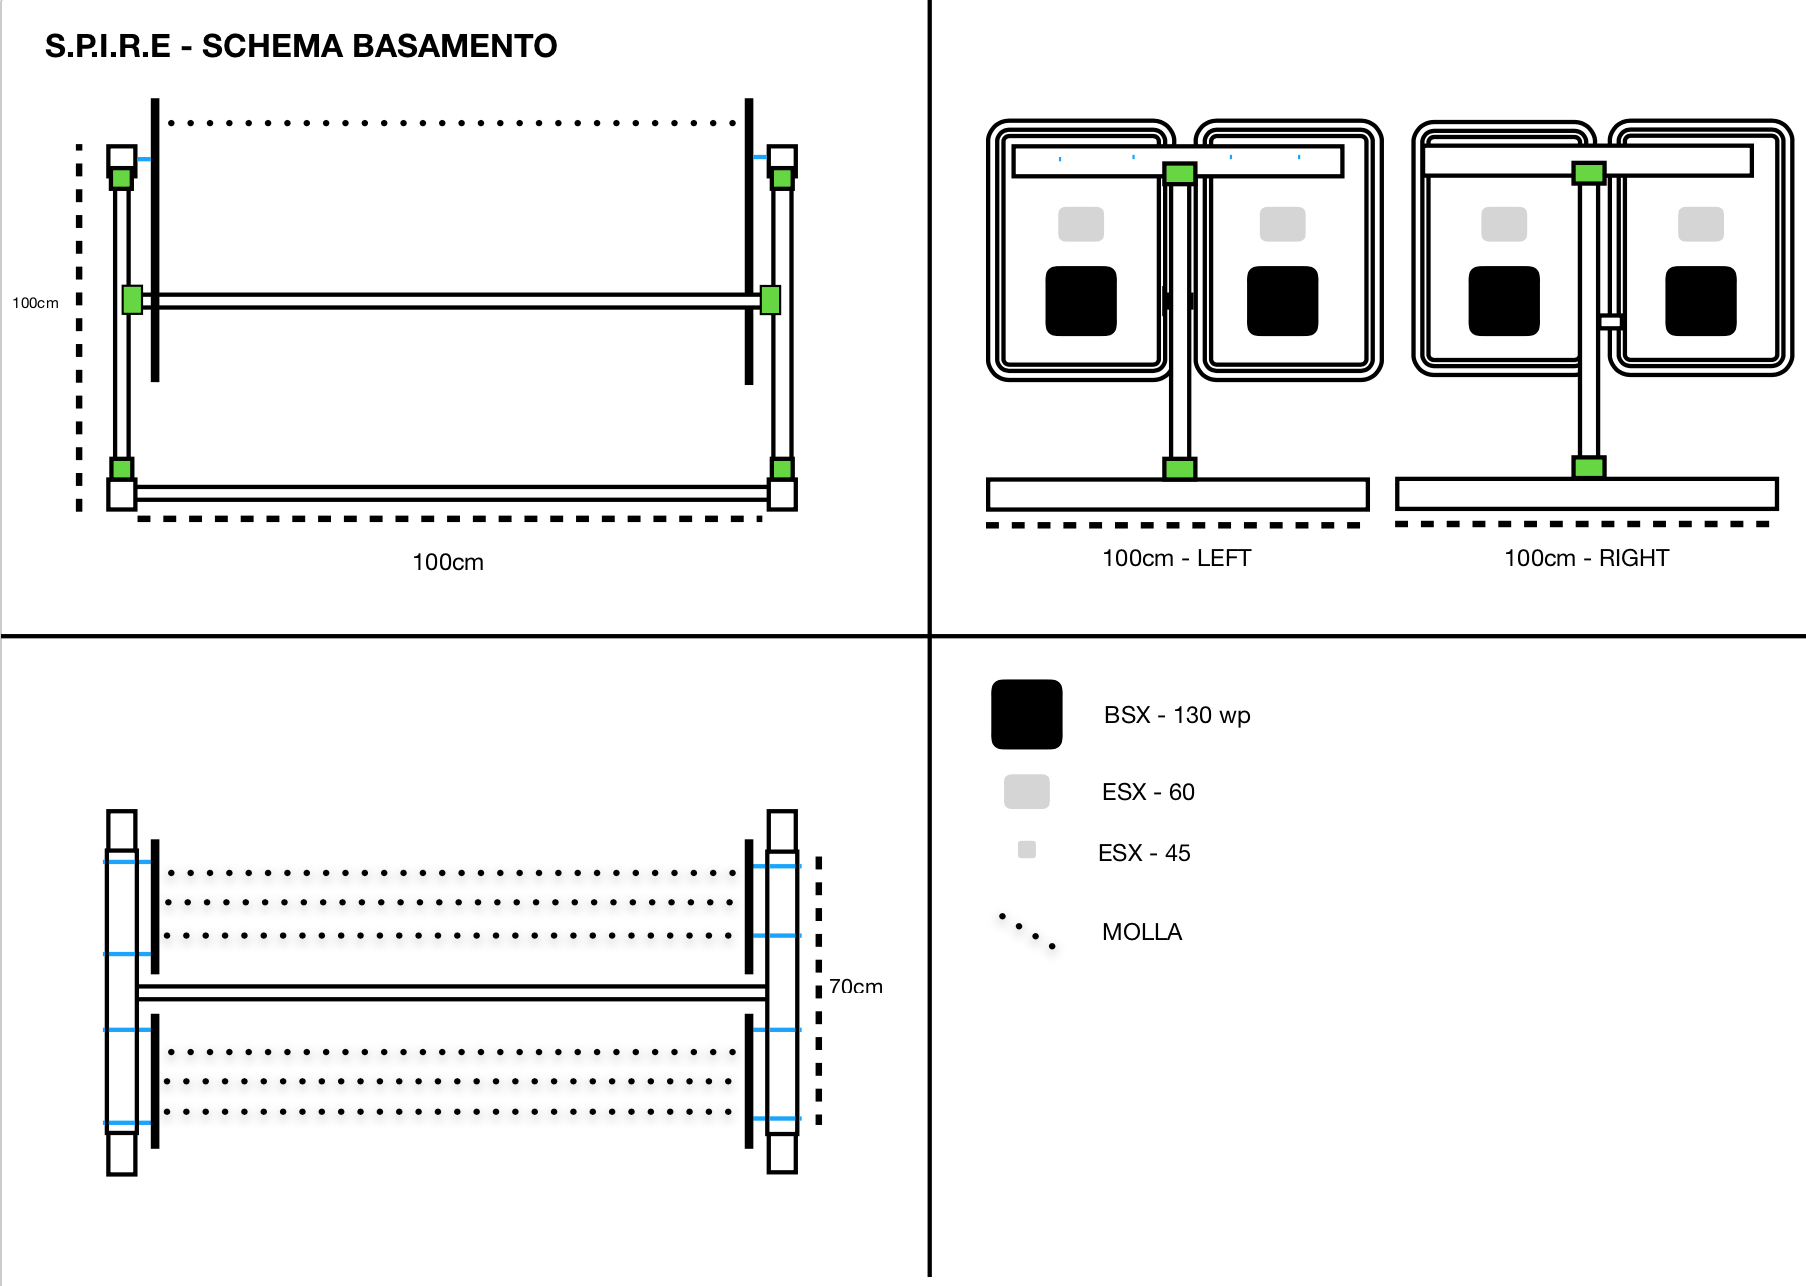
\includegraphics[width=1.\textwidth]{Basamento.jpg}
\end{minipage}
\end{center}

Supporto in ferro. Punti di saldatura in verde. In basso a destra la nomenclatura degli attuatori utilizzati.
In primo luogo la ricerca delle molle. Appena conscio della forma e della natura dello strumento, ho iniziato delle ricerche sulle molle e su le placche (?) in acciaio e ferro armonico. Ho poi contattato il Mollificio Ciullo, ad Albano laziale (Roma) per riuscire ad avere le giuste risposte sulla tipologia delle molle e sul loro funzionamento. Esistono due tipi di molle, del tutto opposte nel loro funzionamento. La natura della molla, a seconda della sua creazione pu� darle delle specifiche del tutto diverso. Le molle prese in esame sono state a (trazione) e a (compressione). 
spiegazione molle a compressione che mi ha portato a visitare un mollificio ad Albano Laziale, il Mollificio Ciullo (\textit{https://www.mollificiociullo.com}) che mi ha esposto le differenze tra le tipologie di molle in commercio e delle peculiarit� elastiche a seconda dei materiali utilizzati. \\
L'acciaio armonico � risultato il materiale migliore per il mio utilizzo perch� a diametri bassi di filatura si possono avere grandi o piccoli diametri per le spire e il risultato non cambia. Ogni molla, se ha un diametro compreso tra 0.1 e 0.2 cm, si ottiene una grande manovrabilit� a livello di flessione e tensione. Da sottolineare che vanno utilizzate solo ed esclusivamente le \underline {Molle a Trazione}; perch� in estensione hanno rigidit� minime anche per lunghezze pari al doppio della loro lunghezza a riposo.
\\
\begin{center}
\begin{minipage}[c]{.7\textwidth}
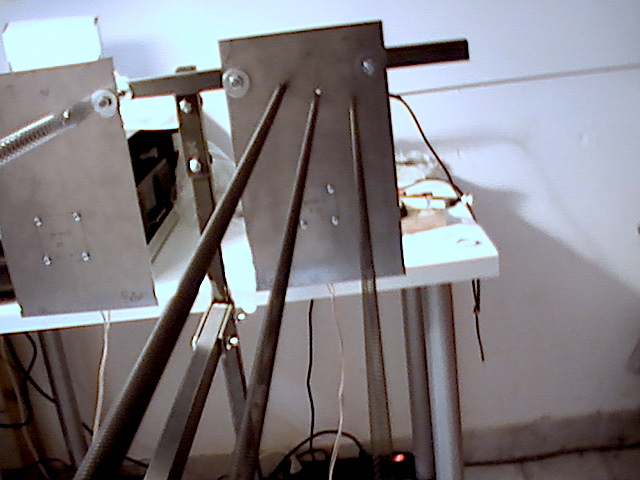
\includegraphics[width=1.\textwidth]{Prototipo2.jpg}
\end{minipage}
\end{center}
Le molle a trazione sono state fissate come in figura, facendo dei buchi sulla lamiera e tese, tutto nella stessa lunghezza, per rendere possibile uno studio omogeneo su materiali diversi che rispondono diversamente al tocco e all'eccitazione mediante attuatori.\\
Si � notato che ogni molla si comporta differentemente a seconda del diametro delle spire, della robustezza del materiale e, ovviamente, del diametro del cavo in acciaio armonico.

\section{Fissaggio Molle e attuatori}
\addcontentsline{toc}{section}{Fissaggio Molle e attuatori}

Gli attuatori sono stati fissati preventivamente tramite del nastro su una delle piastre di metallo e fatte delle prove di risposta del materiale risuonante. Trovato eccellente la risposta del metallo, in questo caso ferro e ferro zigrinato, sono stati segnati dei punti di ancoraggio degli attuatori, tramite viti con rondelle e bulloni. \\ \\
\\
\begin{tabular}{cp{2cm}p{2cm}p{2cm}} \textbf{Tipologia}&\textbf{ATTACCO}&\textbf{BATTENTE}&\textbf{Risposta}\\ 
\hline \textbf{METALLI}\\
\hline Placche metallo&8&Risonatori&Ottima\\
\hline Molle a trazione Inox&2&Strumento&Sufficiente\\
\hline Molle a trazione Acciaio armonico&6&Strumento&Ottima\\
\hline Tubo Quadrato Ferro&2&Basamento&Ottima\\
\hline Viti per innesti&Varie&Bas. Attuatori&Ottima\\
\hline \textbf{MOLLE}\\
\hline BSX 130 WP - 4 Ohm&4&Vibrazione Placca&Ottima\\ 
\hline ESX 45 - 8 Ohm&4&Vibrazione Placca&Sufficiente\\
\hline ESX 60 - 8 Ohm&3&Vibrazione Placca&Buona\\
\hline \textbf{MAGNETI}\\
\hline Humbucker&2&Amplificazione Molle&Buona\\
\hline Double Coil Bass&1&Amplificazione Molle&Ottima\\
\hline \textbf{PIEZOELETTRICI} \\
\hline Piezoelettrici&4&Amplificazione Molle&Buona\\
\hline 
\end{tabular}

\section{Analisi spettrale}
\addcontentsline{toc}{section}{Analisi spettrale}
Di seguito, l'analisi spettrale e lo spettrogramma della risposta all'eccitazione di ogni singola molla. Sottolineo che l'eccitazione della molla, avviene nella parte centrale. \\
\begin{center}
\begin{minipage}[c]{1.\textwidth}
\includegraphics[width=1.\textwidth]{MOLLA1.jpg}
\end{minipage}
\end{center}
\begin{center}
\begin{minipage}[c]{1.\textwidth}
\includegraphics[width=1.\textwidth]{MOLLA2.jpg}
\end{minipage}
\end{center}
\begin{center}
\begin{minipage}[c]{1.\textwidth}
\includegraphics[width=1.\textwidth]{MOLLA3.jpg}
\end{minipage}
\end{center}
\begin{center}
\begin{minipage}[c]{1.\textwidth}
\includegraphics[width=1.\textwidth]{MOLLA4.jpg}
\end{minipage}
\end{center}

Ogni molla � soggetta ad un inviluppo e un decadimento differente, questo porta, a livello compositivo, a gestire sia timbri che dinamiche diverse per lavorare sia sulla parte orizzontale della stesura compositiva che verticale. Gli incastri formali consisteranno, infatti in \textit{crescendo} dinamici legati soprattutto ai rapporti timbrici tra le molle.


\section{Schema Elettrico}
\addcontentsline{toc}{section}{Schema Elettrico}
Di seguito, lo schema elettrico per il collegamento degli attuatori:
\begin{center}
\includegraphics[width=1.\textwidth]{Elettrico.jpg}
\end{center}

